
\begin{figure}
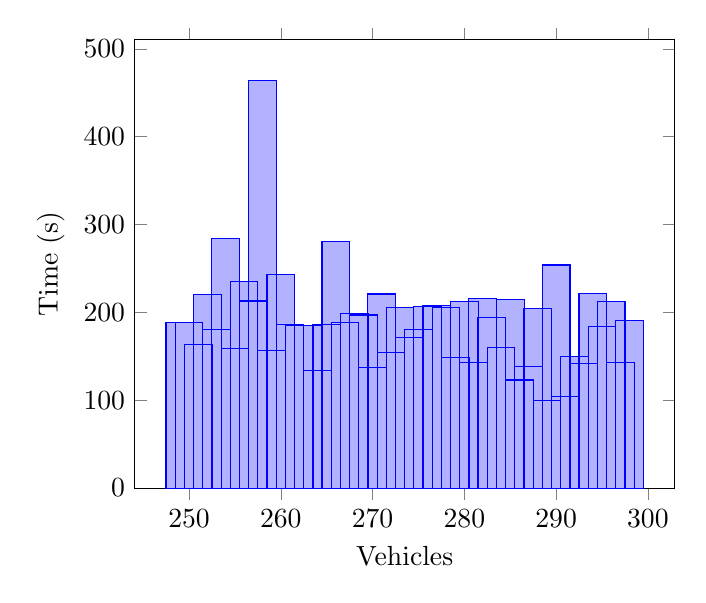
\begin{tikzpicture}
\begin{axis}[
legend style={anchor=west},
xlabel=Vehicles,
ylabel=Time (s),
ymin=0,
ybar,
]
\addplot coordinates {
(298, 191)
(296, 212)
(297, 143)
(295, 184)
(292, 150)
(293, 142)
(290, 254)
(291, 104)
(270, 137)
(271, 221)
(272, 154)
(274, 171)
(275, 181)
(276, 207)
(277, 208)
(278, 206)
(279, 149)
(249, 189)
(294, 222)
(273, 206)
(258, 464)
(259, 157)
(252, 220)
(250, 189)
(251, 163)
(256, 235)
(257, 213)
(254, 284)
(255, 159)
(280, 212)
(289, 100)
(288, 204)
(281, 143)
(283, 194)
(282, 216)
(285, 215)
(284, 160)
(287, 138)
(286, 123)
(263, 185)
(262, 185)
(261, 186)
(260, 243)
(267, 189)
(266, 281)
(265, 186)
(264, 134)
(269, 197)
(268, 199)
(253, 181)
};

\end{axis}
\end{tikzpicture}
\label{tik:time:100:91}
\caption{100 percent diving with GSC on route $91$}
\end{figure}
